\chapter{Rail Network and Train}

This module is responsible for creating the underlying railway network and the trains that run on 
these networks. Railway network module is implemented in \textbf{network.py} and train component is implemented in 
\textbf{train.py}.
\vspace{0.5cm}
\section {Mathematical model}
This mathematical model is from \cite{ARTICLE:2}. The railway network is modelled as a graph
$ \mathcal{G}( \mathcal{N} ,\mathcal{E})$ where $\mathcal{N}$ denotes the set of all nodes, and 
$\mathcal{E}$ denotes
the set of all edges. A set of vehicles $\mathcal{V}$ is to be scheduled
through this network, which implies that vehicles $v_i \in \mathcal{V}$
must be allotted time slots at successive nodes and edges,
such that they can move from their respective origins to
destinations via predefined routes (sequence of nodes). Each
pair of nodes is connected by at most one edge, and thus
routes also define the sequence of edges to be traversed.
Each node $n_j \in \mathcal{N}$ and edge $e_k \in \mathcal{E}$ is assumed to be
composed of one or more parallel (equivalent) resources,
denoted by $r_{m}^{nj}$ and $r_{p}^{ek}$ respectively, where $m \in \{1, \ldots R^{n}_{j}\}$
and $p \in \{1, \ldots R^{e}_{k}\}$.

\vspace{0.25cm}
Let us define the arrival time of a vehicle $v_i$ at node $n_j$ by
$t_{i}^{a} (n_j)$, and its departure time to be $t^{d}_{i} (n_j )$. Complementarily,
the arrival time to and departure time from an edge $e_k$ is
denoted by $t^{a}_{i} (e_k )$ and $t^{d}_{i} (e_k )$ respectively. If $e_k$ is traversed
upon leaving $n_j$ , then $t^{a}_{i}(e_k) = t^{d}_{i} (n_j )$. If the next node
after $e_k$ is $n_{j}^{'}$ , then $t^{d}_{i} (e_k ) = t^{a}_{i} (n_{j}^{'} )$. For simplicity, it is
assumed that all parallel resources at a node are accessible
from all resources at adjoining edges. Finally, we define the
binary variables $b^{nj}_{m}(i)$ and $b_{p}^{ek}(i)$ to be equal to 1 if $v_i$ is
allocated to resources $r_{m}^{nj}$ and $r_{p}^{ek}$ at respective nodes or
edges, and 0 otherwise. Each vehicle $v_i$ has an earliest start
time on its journey (arrival time at first node) given
by $T_i$ , and its computed finishing time (departure from last
node) is denoted by $f_i$ . Its minimum halt time at node $n_j$
is given by $H_i (n_j )$, and minimum travel time on edge $e_k$ is
given by $W_i (e_k )$.

\vspace{0.25cm}
Time constraints, $$t^{d}_{i} (n_{j} ) - t^{a}_{i} (n_{j} ) \geq H_{i} (n_{j} )$$
$$t^{d}_{i} (e_{k} ) - t^{a}_{i} (e_{k} ) \geq W_{i} (e_{k} )$$

Resource Contraints,
$$\sum_{m} b_{m}^{nj}(i) = 1$$
$$\sum_{m} b_{m}^{ek}(i) = 1$$

\section{Railway Network}


Railway network consists of two building blocks \textbf{Stations} and \textbf{Tracks} that connect
stations. All the fields of tracks and stations are given in the diagram below. Railway network is a weighted 
networkx graph where nodes are stations (Station class is added as attribute to the node) and edges are 
tracks running between stations (Track class is added as attribute to the edge). Input is given using two
separate text files, one corresponding to tracks and other corresponding to stations. More detailed info is 
in repository.


\begin{figure}[h]
    \centering
    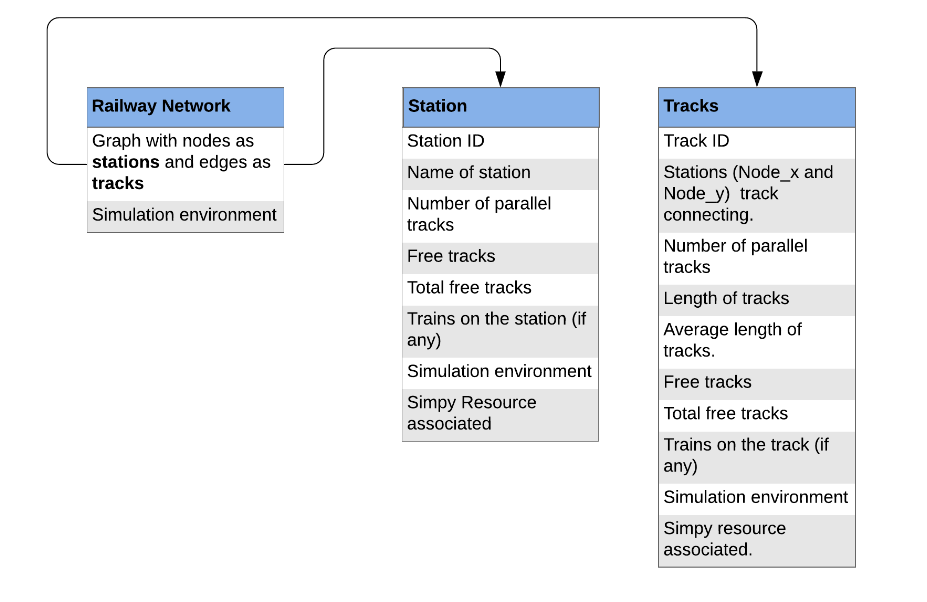
\includegraphics[width=1.0\textwidth]{Rail_train}
    \caption{ Railway Network framework }
    \label{image-myimage2}
\end{figure}

\section{Trains}
There are multiple trains running in the network at a time. Train class defines all the variables and methods
of this class and simulator uses this class to create process corresponding to each train (more details in simulator 
section).

\vspace{0.25cm}
Train movements over the scheduling horizon must be described in one of two ways. The first option is
to define a reference timetable which gives the desired arrival
and departure time of each train at each station. The second
option is to provide the earliest movement times from their
current locations (or origin stations), followed by the minimum
running times (on track sections between stations) and halt
times (at stations) up to the destinations. Note that the running
and halt times can be completely heterogeneous: each train
may have a different running/halt time in each resource,
depending on the length of track, the type of halt, and the
type of locomotive. The timetable can be derived by adding
the running and halt times of each train to the current time.

\begin{figure}[h]
    \centering
    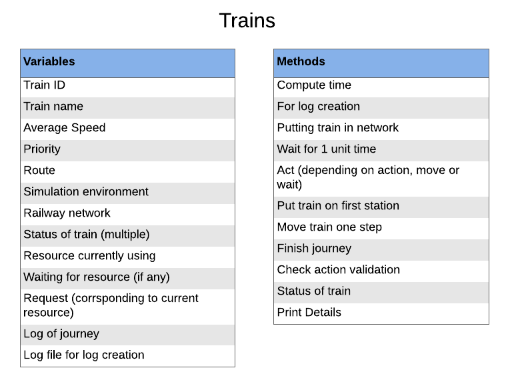
\includegraphics[width=0.8\textwidth]{train}
    \caption{ Train Variables and methods }
    \label{image-myimage3}
\end{figure}

Variables in the train class are self understood. Following are the explanation and implementation details of 
the method. For more details look into the repository where explicit documentation is given.
\begin{enumerate}
\item \textbf{Compute Time} : To calculate the travel time of the train between two stations.
\item \textbf{Log Creation} : To create log corresponding to important events for each train.
\item \textbf{Put train in network} : This method puts the train in the network and generates an event 
                                    corresponding to start time of the train. After start time, train movement is 
                                    controlled using \textbf{Act} method.
\item \textbf{Wait} : To make train wait for predefined unit of time.
\item \textbf{Act} : This method takes one argument, either to move the train or wait. Depending on the 
                    argument, specified action is taken.
\item \textbf{Put train on first station} : This method tries to put the train onto first station and thus 
                            initiating the journey of the train. It may be possible, that the station is not 
                            free, in which case the move is invalid or it waits till the resource is freed.
\item \textbf{Move train one step} : Move the train one step. If the train is on the station, then it will try to 
                                depart to the next track or if the train is on track, then it will try to arrive at the 
                                next station.
\item \textbf{Finish journey} : This method is used when the train is at the last station and it has to 
                                free the last resource.
\item \textbf{Check action validation} : Check wether the given action (move or wait) is valid for the current status of the train.
\item \textbf{Status of train} : To give the current status of the train.
\item \textbf{Print details} : To print the details of the train.
\end{enumerate}

Trains need action only for the following events :
\begin{enumerate}
\item If a train is standing at a station, the event processing time 
    corresponds to the earliest time at which the train can depart,   
    as defined by its minimum halt time at the station and by any     
    departure time constraints enforced for passenger convenience.
\item If it is running between two stations, the event processing time        
    corresponds to the earliest time at which it can arrive at the         
    next station, as defined by the length of the track and the train      
    running speed.

\item  If the train is yet to start, the event processing                      
    time is the time at which it is expected at the starting station. This event is created 
    by \textit{put train in network} method. Once this event is generated, then \textit{put train on 
    first station} is used to put the train on the first station.

\end{enumerate}


Once the train process is running, it is in one of the following states :
\begin {enumerate}
\item Train is not yet started.
\item Train is running in the network.
\item Train has reached the destination( final station in journey) but the resource is not yet freed.
\item Train has completed journey and released all the resources.
\end {enumerate}

This status is used by create statistics process, that terminates the simulation if all the trains have completed it's 
journey.